\chapter{Standard Access Control
Lists}\label{standard-access-control-lists}

WHAT ARE ACLs

\begin{itemize}
\tightlist
\item
  ACLs (Access Control Lists) have multiple uses
\item
  In DAY 34 and DAY 35, we will focus on ACL's from a security
  perspective
\item
  ACLs function as a ``packet filter'' - instructing the ROUTER to ALLOW
  or DENY specific traffic
\item
  ACLs can filter traffic based on:

  \begin{itemize}
  \tightlist
  \item
    SOURCE / DESTINATION IP ADDRESSES
  \item
    SOURCE / DESTINATION LAYER 4 PORTS
  \item
    etc.
  \end{itemize}
\end{itemize}

HOW ACLs WORK

\begin{figure}
\centering
\pandocbounded{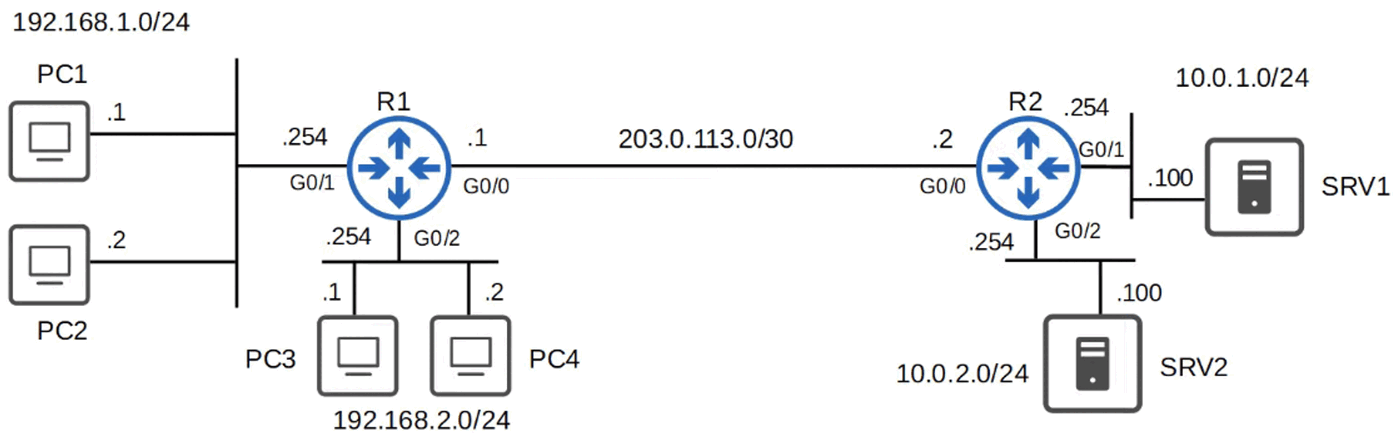
\includegraphics[keepaspectratio,alt={image}]{images/35-standard-access-control-lists/img-001.png}}
\end{figure}

\begin{tipbox}

REQUIREMENTS:

\begin{itemize}
\tightlist
\item
  Hosts in 192.168.1.0/24 should have ACCESS to the 10.0.1.0/24 NETWORK
\item
  Hosts in 192.168.2.0/24 should not have ACCESS to the 10.0.1.0/24
  NETWORK
\end{itemize}

\end{tipbox}

ACLs are configured GLOBALLY on the ROUTER (Global Config Mode)

\begin{itemize}
\tightlist
\item
  They are an ordered sequence of ACEs (Access Control Entries)
\end{itemize}

\begin{figure}
\centering
\pandocbounded{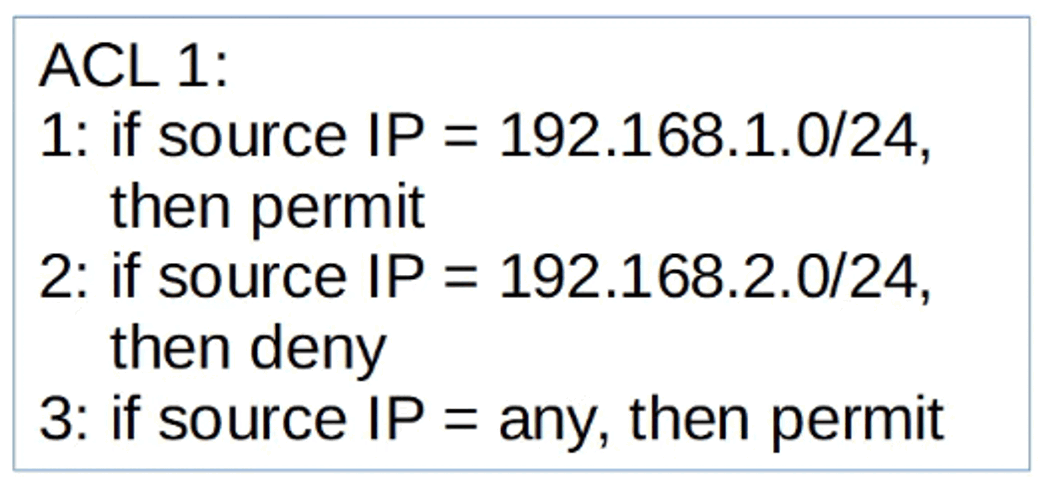
\includegraphics[keepaspectratio,alt={image}]{images/35-standard-access-control-lists/img-002.png}}
\end{figure}

\begin{itemize}
\tightlist
\item
  Configuring an ACL in Global Config Mode will not make the ACL take
  effect
\item
  The ACL must be applied to an interface

  \begin{itemize}
  \tightlist
  \item
    ACLs are applied either INBOUND or OUTBOUND
  \end{itemize}
\item
  ACLs are made up of one or more ACEs
\item
  When a ROUTER checks a PACKET against the ACL, it processes the ACEs
  in order, from top to bottom
\item
  If the PACKET matches one of the ACEs in the ACL, the ROUTER takes the
  action and stops processing the ACL. All entries below the matching
  entry will be ignored
\end{itemize}

\begin{figure}
\centering
\pandocbounded{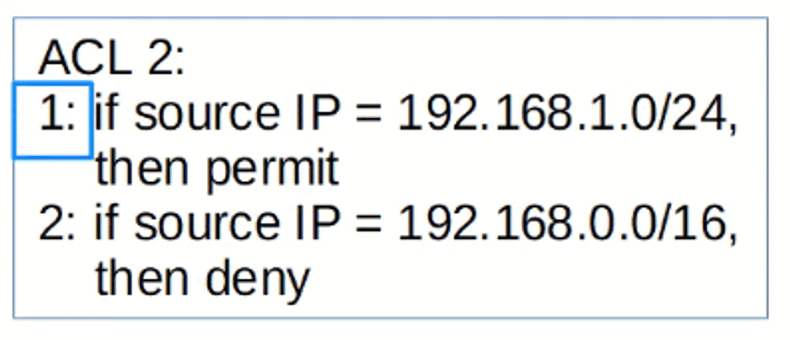
\includegraphics[keepaspectratio,alt={image}]{images/35-standard-access-control-lists/img-003.png}}
\end{figure}

\begin{figure}
\centering
\pandocbounded{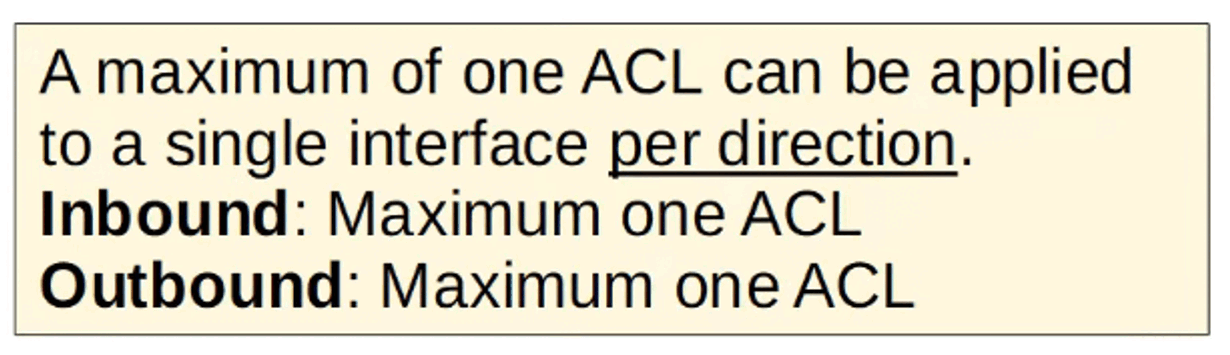
\includegraphics[keepaspectratio,alt={image}]{images/35-standard-access-control-lists/img-004.png}}
\end{figure}

\section{Implicit Deny}\label{implicit-deny}

\begin{itemize}
\tightlist
\item
  What will happen if a PACKET doesn't match any of the entries in an
  ACL ?
\item
  There is an INPLICIT DENY at the end of ALL ACL's
\item
  The IMPLICIT DENY tells the ROUTER to DENY ALL TRAFFIC that doesn't
  match ANY of the configured entries in the ACL
\end{itemize}

\section{ACL Types}\label{acl-types}

\begin{figure}
\centering
\pandocbounded{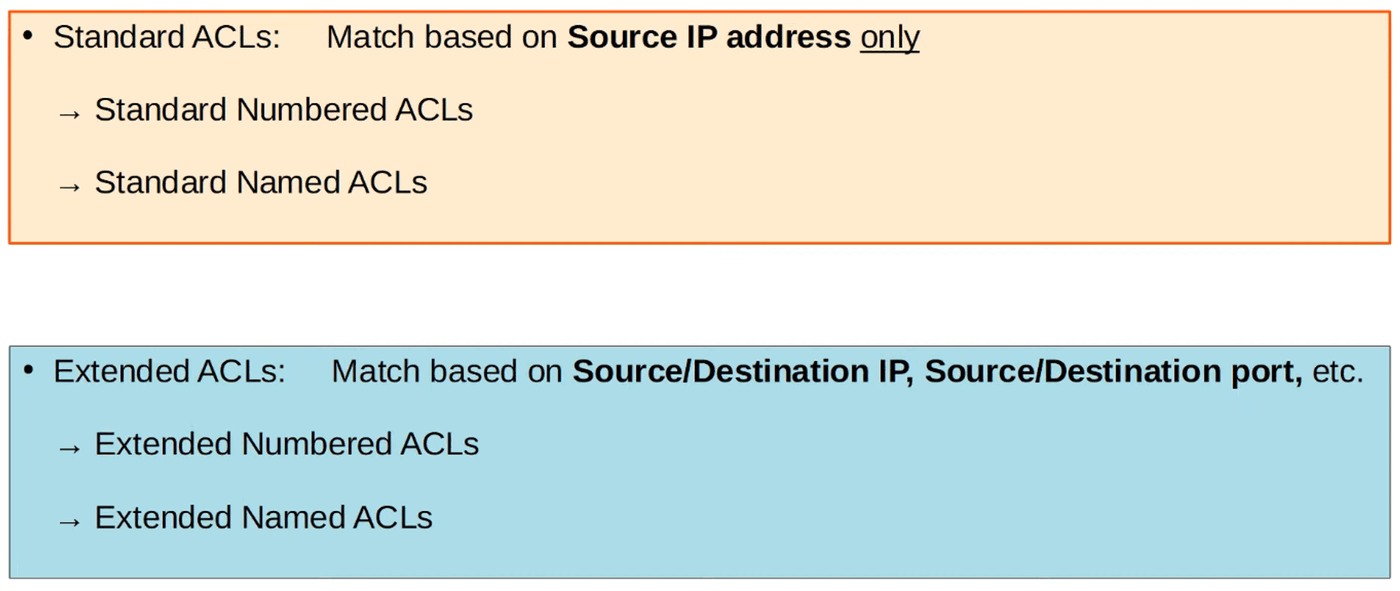
\includegraphics[keepaspectratio,alt={image}]{images/35-standard-access-control-lists/img-005.png}}
\end{figure}

STANDARD NUMBERED ACLs

\begin{itemize}
\tightlist
\item
  Match traffic based only on the SOURCE IP ADDRESS of the PACKET
\item
  Numbered ACLs are identified with a number (ie: ACL 1, ACL 2, etc.)
\item
  Different TYPES of ACLs have a different range of numbers that can be
  used
\end{itemize}

\begin{tipbox}

STANDARD ACLs can use 1-99 and 1300-1999

\end{tipbox}

\begin{itemize}
\item
  The basic command to configure a STANDARD NUMBERED ACL

  \begin{itemize}
  \tightlist
  \item
    \passthrough{\lstinline!R1(config)\# access-list *number* \{deny | permit\} *ip wildcard-mask*!}
  \end{itemize}

  This is an example of denying a SPECIFIC host's traffic

  REMEMBER : 0.0.0.0 wildcard is the same as 255.255.255.255 or a /32
  host

  \begin{itemize}
  \tightlist
  \item
    Example :
    \passthrough{\lstinline!R1(config)\# access-list 1 deny 1.1.1.1 0.0.0.0!}
  \item
    Example :
    \passthrough{\lstinline!R1(config)\# access-list 1 deny 1.1.1.1!}(identical
    to the above)
  \item
    Example :
    \passthrough{\lstinline!R1(config)\# access-list 1 deny host 1.1.1.1!}
  \end{itemize}

  If you want to permit ANY traffic from ANY source

  \begin{itemize}
  \tightlist
  \item
    Example :
    \passthrough{\lstinline!R1(config)\# access-list 1 permit any!}
  \item
    Example :
    \passthrough{\lstinline!R1(config)\# access-list 1 permit 0.0.0.0 255.255.255.255!}
  \end{itemize}

  If you want to make a description for a specific ACL

  \begin{itemize}
  \tightlist
  \item
    Example :
    \passthrough{\lstinline!R1(config)\# access-list 1 remark \#\# BLOCK BOB FROM ACCOUNTING \#\#!}
  \end{itemize}
\end{itemize}

\begin{figure}
\centering
\pandocbounded{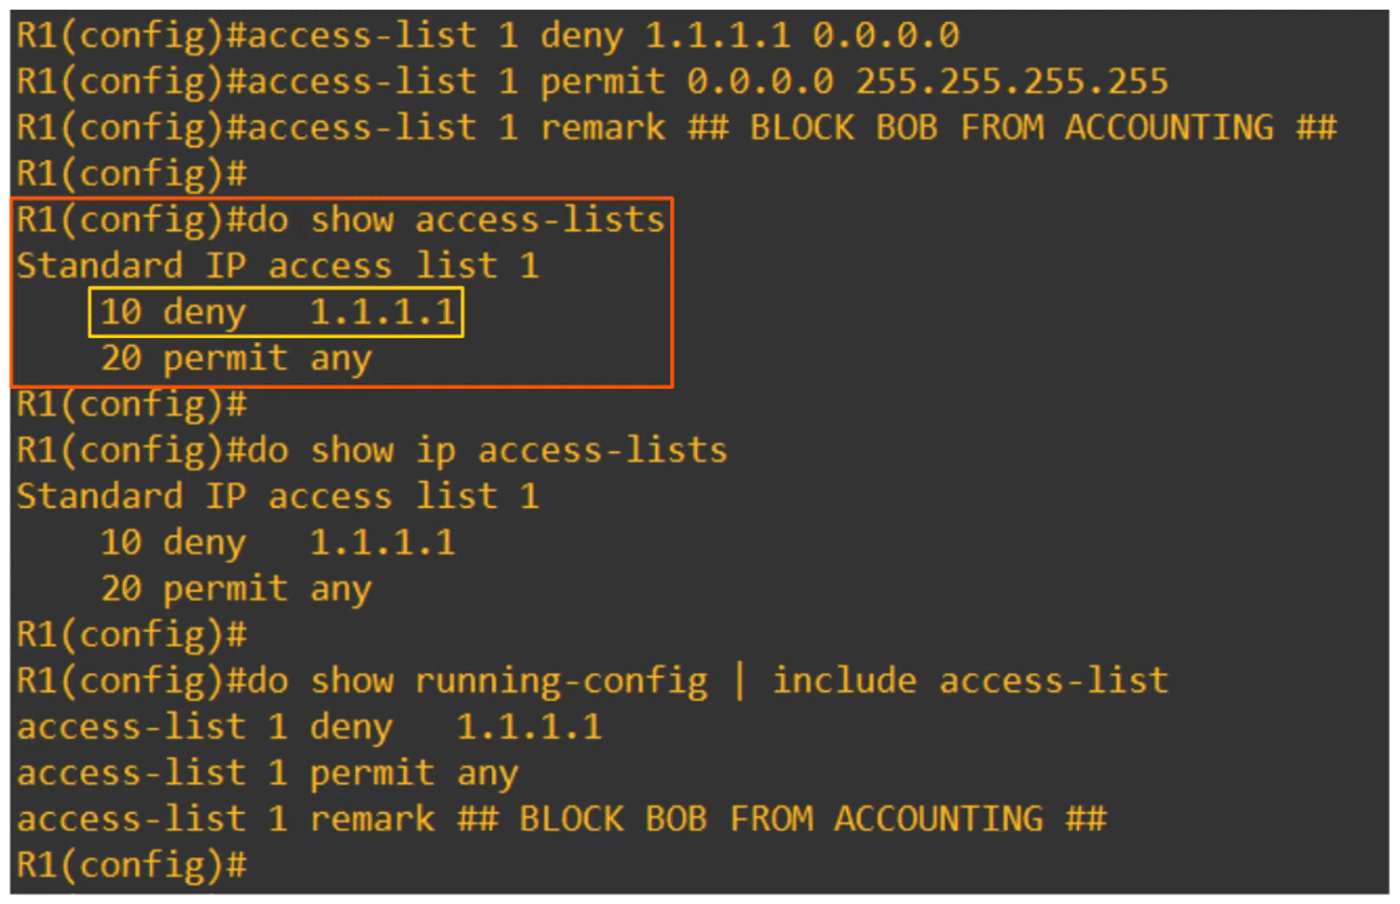
\includegraphics[keepaspectratio,alt={image}]{images/35-standard-access-control-lists/img-006.png}}
\end{figure}

Order is important. Lower Numbers are processed FIRST

\section{To Apply an ACL to an
Interface}\label{to-apply-an-acl-to-an-interface}

\passthrough{\lstinline!R1(config-if)\# ip access-group *number* \{in | out\}!}

\begin{figure}
\centering
\pandocbounded{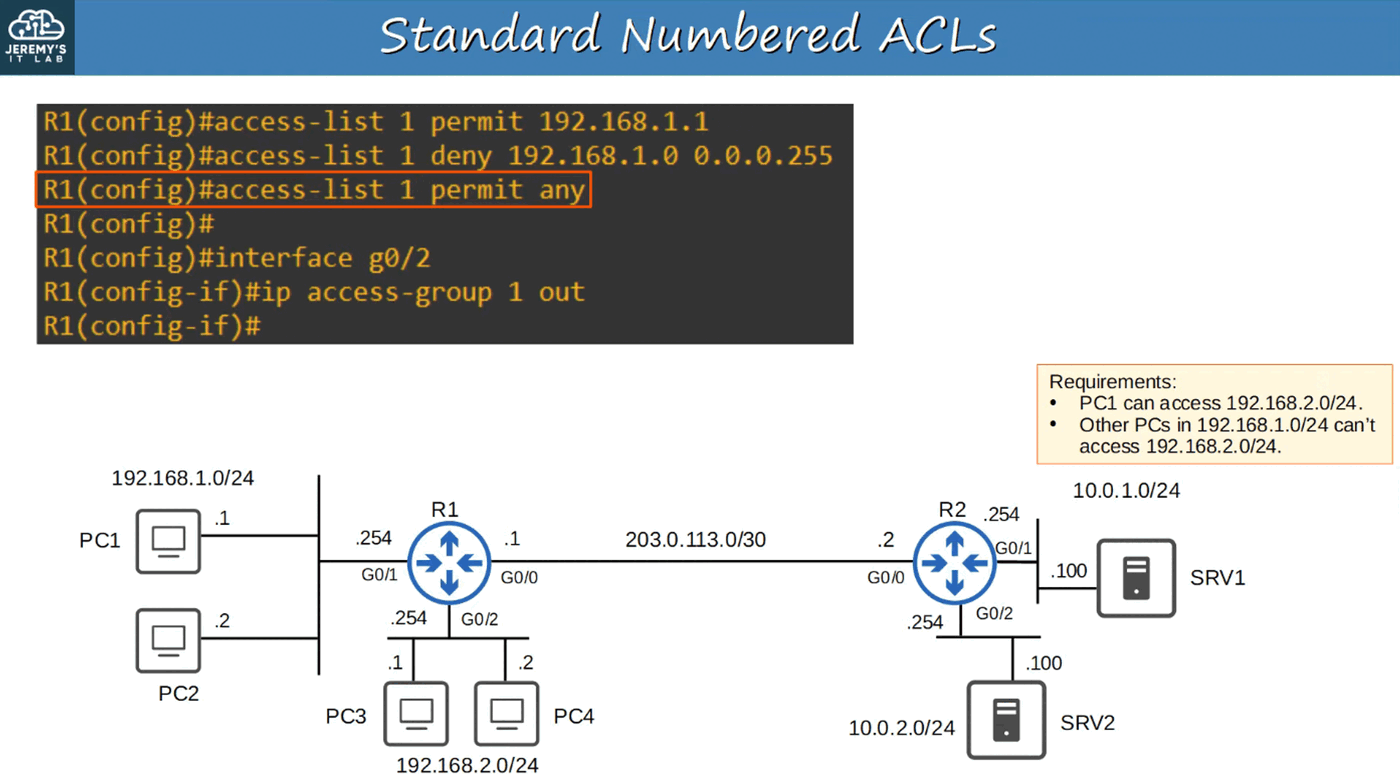
\includegraphics[keepaspectratio,alt={image}]{images/35-standard-access-control-lists/img-007.png}}
\end{figure}

WHY WAS THIS RULE PLACED ON G0/2 OUT ?

\begin{tipbox}

STANDARD ACLs should be applied as CLOSE to the DESTINATION as possible!

\end{tipbox}

STANDARD NAMED ACLs

\begin{itemize}
\tightlist
\item
  Standard ACLs match traffic based only on the SOURCE IP ADDRESS of the
  PACKET
\item
  NAMED ACLs are identified with a NAME (ie: `BLOCK\_BOB')
\item
  STANDARD NAMED ACLs are configured by entering `standard named ACL
  config mode' then configuring EACH entry within that config mode

  \begin{itemize}
  \tightlist
  \item
    \passthrough{\lstinline!R1(config)\# ip access-list standard *acl-name*!}
  \item
    \passthrough{\lstinline!R1(config-std-nacl)\# [*entry-number*] \{deny | permit\} *ip wildcard-mask*!}
  \end{itemize}
\end{itemize}

\begin{figure}
\centering
\pandocbounded{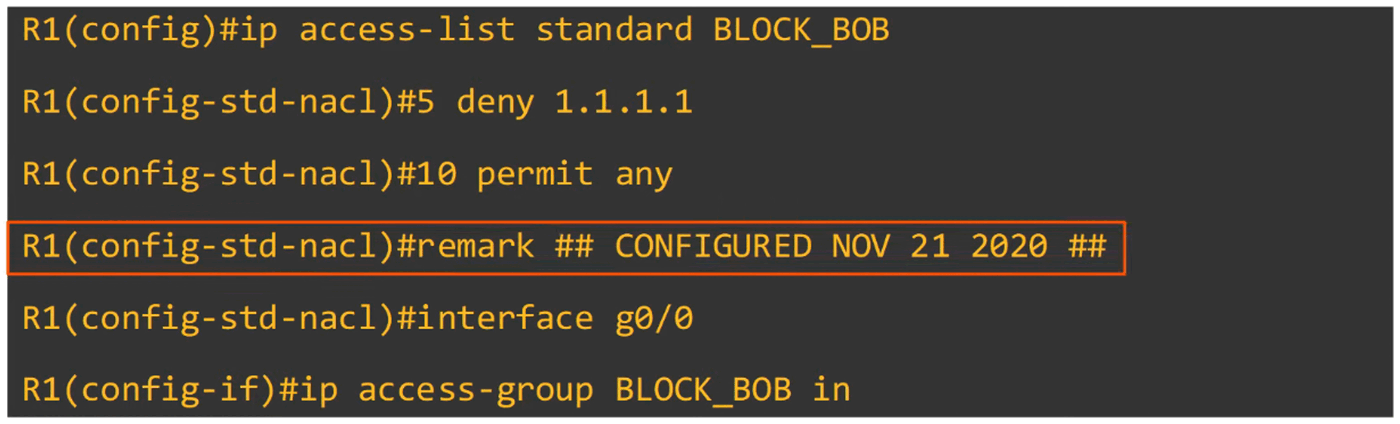
\includegraphics[keepaspectratio,alt={image}]{images/35-standard-access-control-lists/img-008.png}}
\end{figure}

\begin{figure}
\centering
\pandocbounded{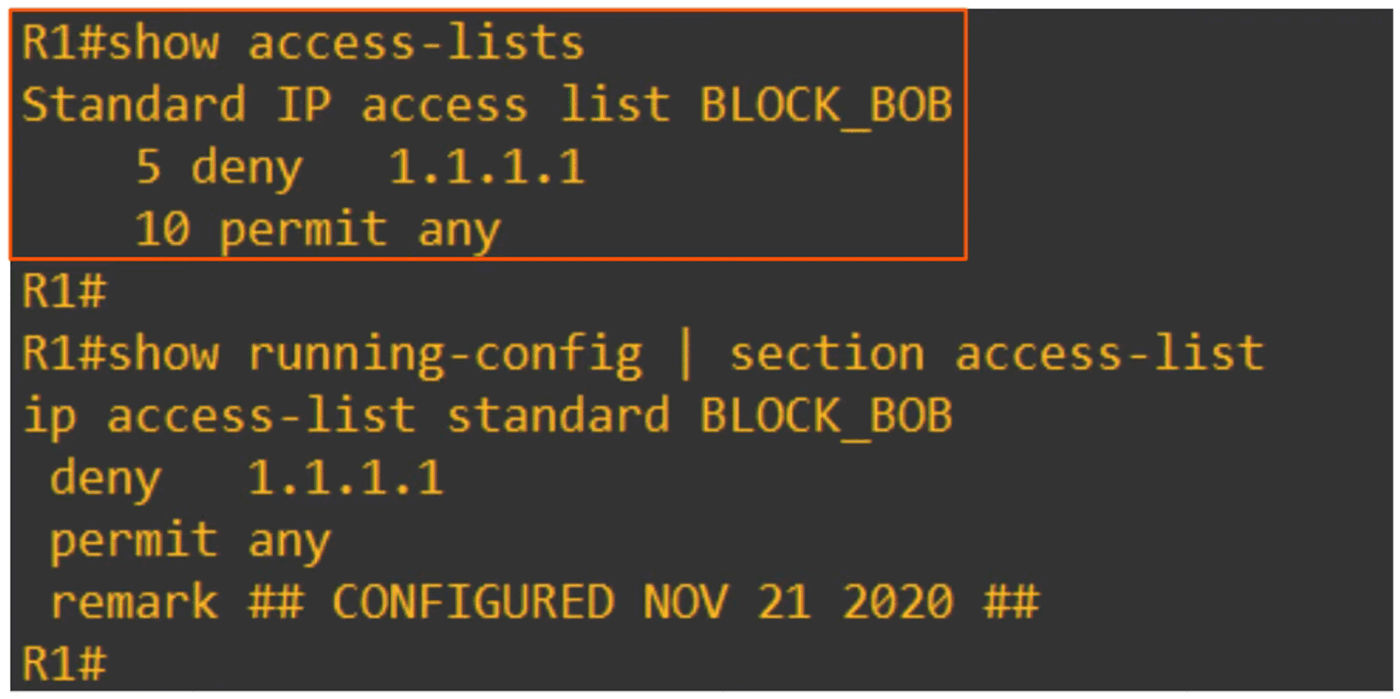
\includegraphics[keepaspectratio,alt={image}]{images/35-standard-access-control-lists/img-009.png}}
\end{figure}

\begin{figure}
\centering
\pandocbounded{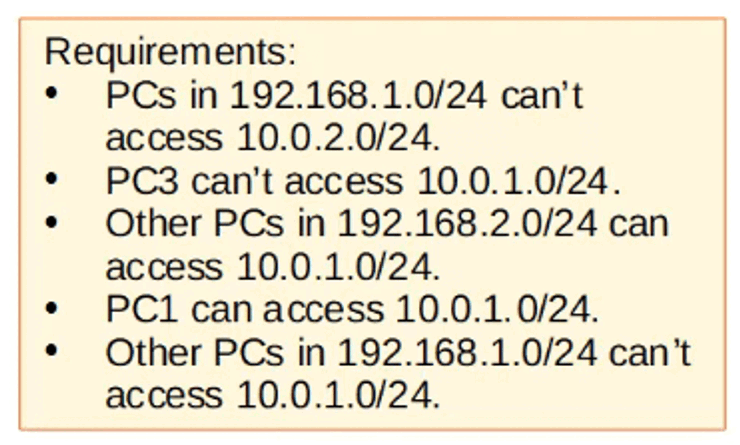
\includegraphics[keepaspectratio,alt={image}]{images/35-standard-access-control-lists/img-010.png}}
\end{figure}

\begin{figure}
\centering
\pandocbounded{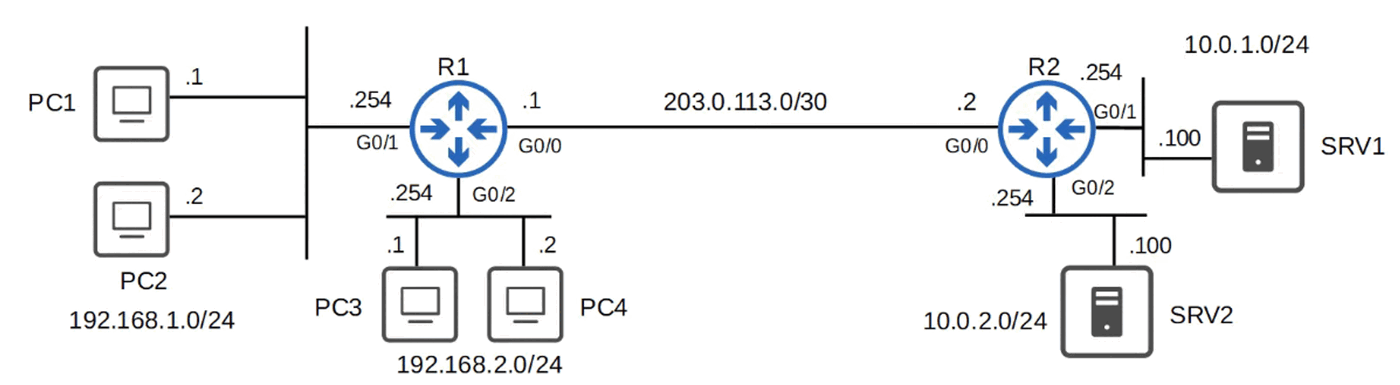
\includegraphics[keepaspectratio,alt={image}]{images/35-standard-access-control-lists/img-011.png}}
\end{figure}

Here are the configurations for the above:

\begin{figure}
\centering
\pandocbounded{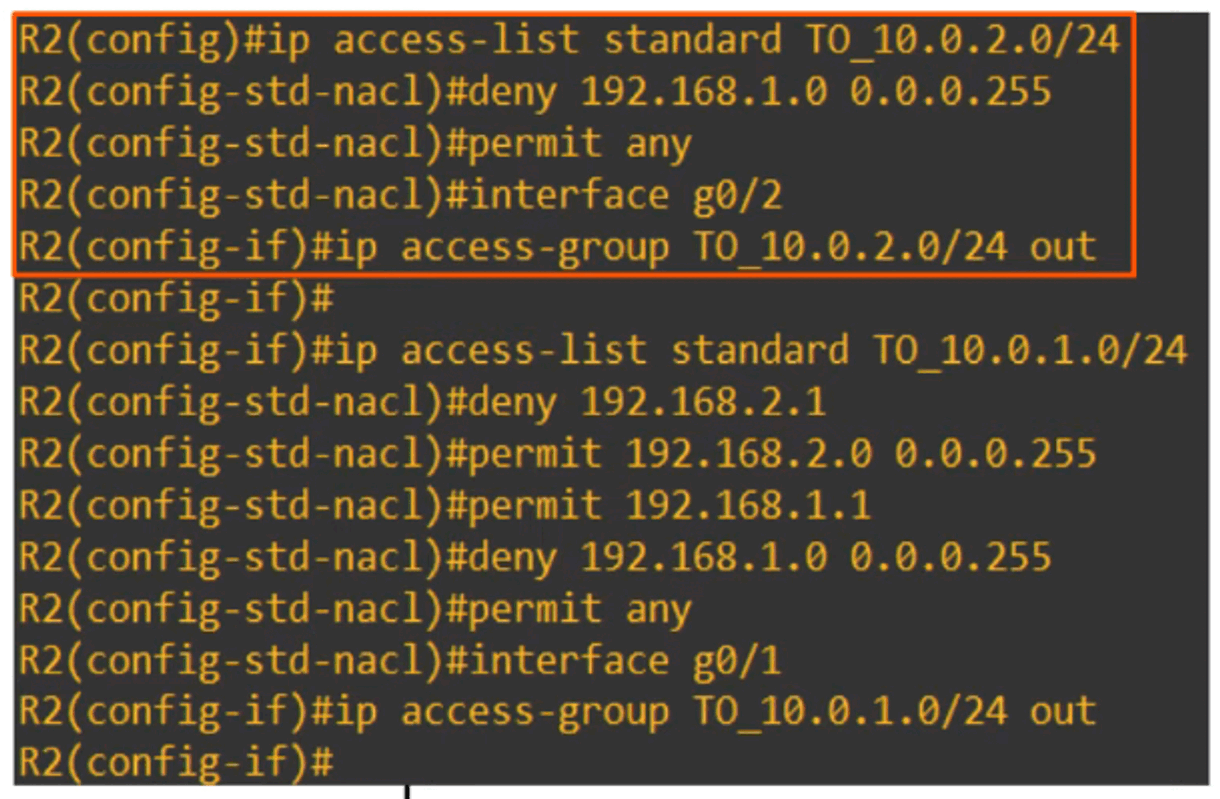
\includegraphics[keepaspectratio,alt={image}]{images/35-standard-access-control-lists/img-012.png}}
\end{figure}

Note, however, how the order is when viewing the ACLs

\begin{figure}
\centering
\pandocbounded{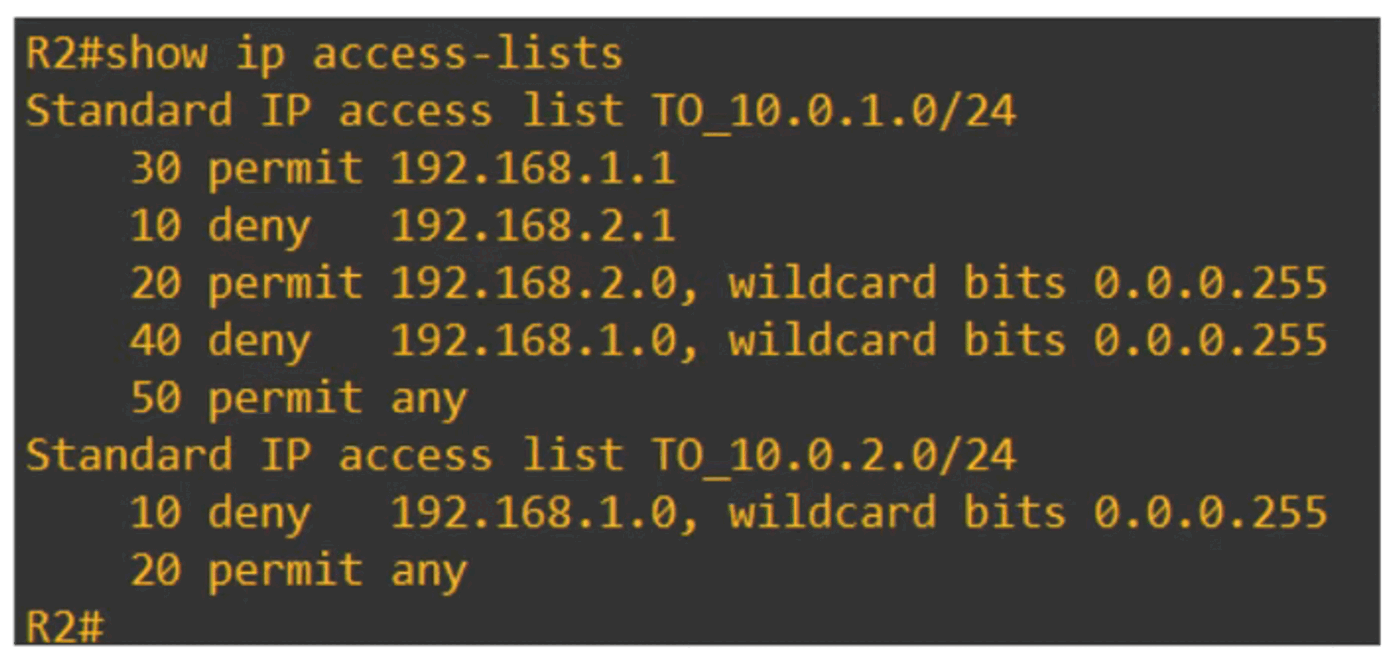
\includegraphics[keepaspectratio,alt={image}]{images/35-standard-access-control-lists/img-013.png}}
\end{figure}

WHY THE REORDERING?

\begin{figure}
\centering
\pandocbounded{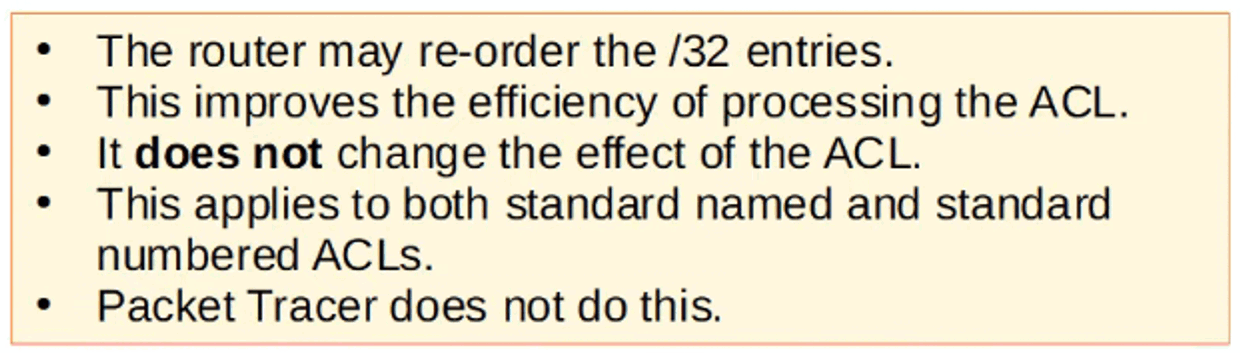
\includegraphics[keepaspectratio,alt={image}]{images/35-standard-access-control-lists/img-014.png}}
\end{figure}

CISCOs PACKET TRACER does not reorder these, however.
